Con la aparici\'on de las computadoras, han ganado espacio dentro de las ciencias naturales los m\'etodos de simulaci\'on.
El uso de estas t\'ecnicas permite validar modelos te\'oricos as\'i c\'omo tambien brindar informaci\'on detallada (microsc\'opica) del proceso simulado.

En el \'ambito de la qu\'imica existen diferentes modelos que permiten simular procesos de interes.
Dentro de estos modelos hay dos que se destacas por su uso.
Los m\'etodos basados en la mec\'anica cu\'antica que proporcionan un a descripci\'on de la estructura electr\'onica del sistema y los m\'etodos basados en la mec\'anica molecular donde las mol\'eculas son tratadas mediante un campo de fuerza
cl\'asico y los electrones no son tenidos en cuenta explicitamente.

\section{Modelos Cu\'anticos (QM)}

El comportamiento de las part\'iculas livianas (c\'omo el electr\'on) est\'a regido por las leyes de la mec\'anica cu\'antica.
Este marco te\'orico desarrollado a comienzos del siglo XX propone que las part\'iculas (c\'omo electrones y protones) pueden (y deben en algunos casos)
ser descriptas c\'omo ondas. As\'i, cualquier propiedad de un sistema esta determinado por una funci\'on llamada funci\'on de onda ($\Psi$) que satisface la ecuaci\'on de Schr\"{o}dinger dependiente del tiempo.

\begin{equation}
    \label{schro_time_dep}
    -\hbar\frac{\partial \Psi}{\partial t} (\mathbf{r},t) = \frac{-\hbar^2}{2\mu}\nabla^2 \Psi(\mathbf{r},t) + V(\mathbf{r},t) \Psi(\mathbf{r},t)
\end{equation}

donde $\mathbf{r} = (r_1,\dots,r_n)$ es el vector de todas las posiciones de las part\'iculas del sistema,
$m$ es la masa de una part\'icula cualquiera, $V$ es un campo externo que afecta a las part\'iculas y
$\hbar$ es la constante de Planck divida por $2\pi$. Si el campo externo no depende del tiempo esta ecuaci\'on se puede simplificar a

\begin{equation*}
    \hat{H} =  -\frac{\hbar^2}{m} \nabla^2 + \hat{V}
\end{equation*}

a la ecuaci\'on de Schr\"{o}dinger \textit{independiente del tiempo}

\begin{equation}
    \label{schro_time_indep}
    \hat{H} \Psi(\mathbf{r}) = E \Psi(\mathbf{r})
\end{equation}

Donde $E$ es la energ\'ia asociada a la funci\'on de onda $\Psi$.

Ahora, si bien resolver esta ecuaci\'on diferencial ser\'ia suficiente para determinar todas las propiedades del sistema, esto no puede hacerse de
manera exacta cuando hay m\'as de un electr\'on en el mismo. Por este motivo, para problemas de mayor tama\~no se utilizan aproximaciones
para obtener una soluci\'on de~\ref{schro_time_indep}.

Existen diversos m\'etodos para resolver (aproximadamente) esta ecuaci\'on con diferente costo computacional (es decir, cantidad de operaciones a realizar)
y calidad de la respuesta obtenida. Dentro de estos m\'etodos hay uno que destaca por su excelente relaci\'on costo/calidad, el m\'etodo basado en la Teor\'ia de los Funcionales de la Densidad
(DFT, Density Functional Theory) desarrollada por Hohenberg y Kohn en 1964.

En este merco te\'orico la \textit{densidad electr\'onica} $\rho$, que representa la probabilidad de encontrar un electr\'on en
el espacio dada una configuraci\'on del sistema ocupa un rol destacado.
La base de este m\'etodo consiste en dos teoremas publicados por Hohenberg y Kohn ~\cite{HohenbergKohn}.
Estos autores demuestran que $\rho$ y $V$ (y por lo tanto $\psi$) se encuentran relacionadas biunivocamente,
es decir que una dada densidad electr\'onica contiene la misma informaci\'on que la funci\'on de onda.
De esta manera cualquier observable (c\'omo la energ\'ia) puede ser representado c\'omo un funcional de la densidad (de all\'i su nombre).

Adem\'as propusieron la dependencia de la energ\'ia del sistema c\'omo funcional de la densidad de la siguiente forma:
\begin{equation}
    \label{hohenberg_kohn_energy}
    E[\rho] = T_s[\rho] + V_{ne}[\rho] + \frac{1}{2} \int \int \frac{\rho(\vec{r}_1) \rho(\vec{r}_2)}{r_{12}} d\vec{r}_1 d\vec{r_2} + E_{xc}[\rho]
\end{equation}

Donde $T_s[\rho]$ es la energ\'ia cin\'etica asociada con la densidad, $V_{ne}[\rho]$ es la energ\'ia potencial producto de la interacci\'on entre los
electrones (la densidad) y los n\'ucleos, el tercer t\'ermino es el resultado de la repulsi\'on de Coulomb entre electrones y $E_{xc}[\rho]$ es la
energ\'ia de intercambio y correlaci\'on. Este \'ultimo t\'ermino da cuenta de la energ\'ia asociada a escribir la funci\'on de onda de manera que cumpla con el principio de antisimetr\'ia de Pauli y de la correlaci\'on
en la posici\'on instant\'anea de los electrones.

Esta formulaci\'on es exacta si se conociera el t\'ermino $E_{xc}[\rho]$ dado que los dem\'as tienen soluci\'on anal\'itica. En las aproximaciones hechas para calcular el mismo reside tanto la calidad c\'omo el costo
computacional de este tipo de simulaciones. Por ello, el objetivo central de este trabajo consiste en mejorar el tiempo insumido en el computo de este t\'ermino.

La forma comunmente utilizada para calcular este t\'ermino se basa en definir un funcional local $\epsilon_{xc}$ que depende de la densidad (Local Density Aproximation, LDA) o de la densidad y su gradiente
(General Gardient Aproximation, GGA) en cada punto del espacio.

De esta manera se puede calcular $ E_{XC} $ mediante la integral:

\begin{equation}
    E_{XC} = \int \rho(r) \epsilon_{xc}\left( \rho(r) \right ) dr
\end{equation}

que es aproximada mediante una suma utilizando una grilla de puntos seg\'un:

\begin{equation}
    \label{approx_excenergy}
    E_{XC} \approx \sum_j \rho(r_j) \epsilon_{xc} (\rho(r_j))
\end{equation}

Otro aspecto importante de esta teor\'ia es que provee una manera de calcular la densidad $\rho$,
mediante el denominado m\'etodo de Kohn-Sham~\cite{KohnSham}. Este m\'etodo se basa en el segundo teorema
de Hohenberg y Khon, que establece que la densidad electr\'onica es la funci\'on que
cumple que $\int \rho(r) dr = N$, la cantidad de \'atomos del sistema, $\rho(r) \geq 0$ y que
minimiza la energ\'ia $E[\rho]$~\ref{hohenberg_kohn_energy}. Esto produce
un m\'etodo auto-consistente para calcular $\rho$. Se empieza con una aproximaci\'on inicial y
se itera el c\'alculo de la misma usando una matriz, denominada \textit{Matriz de Kohn Sham}, hasta
alcanzar un m\'inimo para $E$.

El algoritmo que se deduce de la DFT es uno de los m\'etodos m\'as populares en c\'alculos
de estado s\'olido, especialmente desde la d\'ecada del 90 cuando se mejoraron las aproximaciones para modelado de
interacciones. El valor de esta teor\'ia para el estudio de las propiedades de la materia le vali\'o a Kohn el Premio Nobel
de Qu\'imica en 1998.

Si bien la relaci\'on costo calidad de este m\'etodo es muy buena, el costo computacional asociado sigue siendo elevado lo que limita su aplicaci\'on a sistemas peque\~nos (digamos cientos de \'atomos como m\'aximo).


Por ello se han desarrollado los m\'etodos llamado de mec\'anica molecular (MM). En estos m\'etodos los \'atomos son tratados c\'omo esferas cargadas y las uniones qu\'imicas como resortes (potenciales arm\'onicos).
De esta manera los electrones no son tratados expl\'icitamente lo que reduce dr\'asticamente el consto computacional asociado. Esta t\'ecnica permite es muy poderosa para representar sistemas (o procesos) en los que no cambia la distribuci\'on
electr\'onica.

Sin embargo en muchos de los problemas de inter\'es en qu\'imica y bioqu\'imica (por ejemplo una reacci\'on qu\'imica en soluci\'on o en el seno de una prote\'ina)
 el modelado requiere de la representaci\'on de miles de \'atomos y un tratamiento expl\'icito de los electrones a la vez.

Para resolver esto, se han desarrollado t\'ecnicas h\'ibridas QM/MM (\textit{Quantum Mechanical / Molecular Mechanical}).

Dentro de este esquema se subdivide el sistema en dos. El primero, donde la estructura electr\'onica cambia, se lo modela usando mec\'anica cu\'antica mientras que al resto se le aplica un campo de
fuerzas cl\'asico. De esta manera se puede expresar la energ\'ia de el sistema QM/MM c\'omo.

\begin{equation}
    E = E_{QM} + E_{QM/MM} + E_{MM}
\end{equation}

Donde la energ\'ia $E_{QM}$ se obtiene mediante el m\'etodo DFT visto m\'as arriba, y la energ\'ia
$E_{MM}$ proviene de simular el campo de fuerzas cl\'asico.

La contribuci\'on $E_{QM/MM}$ en este trabajo, se calcula mediante la ecuaci\'on

\begin{equation}
    E_{QM/MM} = \sum_{l = 1}^{N_c} q_l \int \frac{\rho(r)}{\mid r - R_l \mid} + \sum_{l = 1}^{N_c}\sum_{\alpha = 1}^{N_q} [ v_{LJ} ( \mid R_l - \tau_\alpha \mid ) + \frac{q_l z_\alpha}{\mid R_l - \tau_\alpha \mid} ]
\end{equation}

Donde el primer t\'ermino relaciona una carga puntual del sistema cl\'asico con la densidad
electr\'onica, y el segundo t\'ermino representa la interacci\'on entre los n\'ucleos cl\'asicos
con los cu\'anticos mediante un potencial de Lennard-Jones y la interacci\'on Coulombica entre
las cargas.

Los m\'etodos \textit{QM/MM}, dentro del marco de m\'etodos multiescala, son ampliamente utilizados en
la pr\'actica. Estos modelos han valido a Karplus, Levitt y
Warshel el premio Nobel de Qu\'imica en 2013, por su valor para la simulaci\'on de sistemas complejos.

Nuestro trabajo se realiza en base a programas ya existentes. El c\'alculo de $E_{QM}$ y $E_{QM/MM}$ son realizados por el paquete de
\textit{software} LIO~\cite{LIO}~\cite{TesisNitsche}, el cual fue optimizado en este trabajo para el uso de
distintas arquitecturas de CPU y GPGPU. Esta librer\'ia
se complementa mediante el uso del programa de din\'amica molecular Amber~\cite{Amber}, que realiza el c\'alculo
de $E_{MM}$. Nos concentraremos en las partes computacionalmente m\'as intensivas de LIO, que corresponden a la
implementaci\'on de los c\'alculos de los t\'erminos de intercambio y correlaci\'on introducidos en esta secci\'on.

\section{C\'omputo de alto rendimiento}

Una parte significativa del impacto de las computadoras en los distintos aspectos de las ciencias, incluso de la vida diaria, se debe al crecimiento de su poder de c\'omputo desde la aparici\'on de los primeros microprocesadores hasta los disponibles hoy en d\'ia.

Entre 1986 y 2002, la performance de los procesadores creci\'o, en promedio, un $50\%$ por a\~no~\cite{Pacheco}, en parte gracias a la denominada \textit{Ley de Moore}, que
establec\'ia que la densidad de transistores por circuito integrado se duplicaba cada 18 meses~\cite{HennessyPatterson}.
Esto puede verse en la figura~\ref{moore-law}, que compara la cantidad de transistores de distintos procesadores desde 1971 a la actualidad.

Este crecimiento constante permiti\'o a los desarrolladores de procesadores incrementar la potencia de c\'alculo, duplicando la performance cada 24 meses.
Esto benefici\'o durante mucho tiempo a los desarrolladores de aplicaciones, quienes escrib\'ian programas secuenciales, que solo deb\'ian esperar a la aparici\'on de los nuevos modelos de procesadores para ver una reducci\'on sustancial en los tiempos de ejecuci\'on de sus aplicaciones (fen\'omeno denominado \textit{hardware free lunch}).

\begin{figure}[htbp]
   \centering
   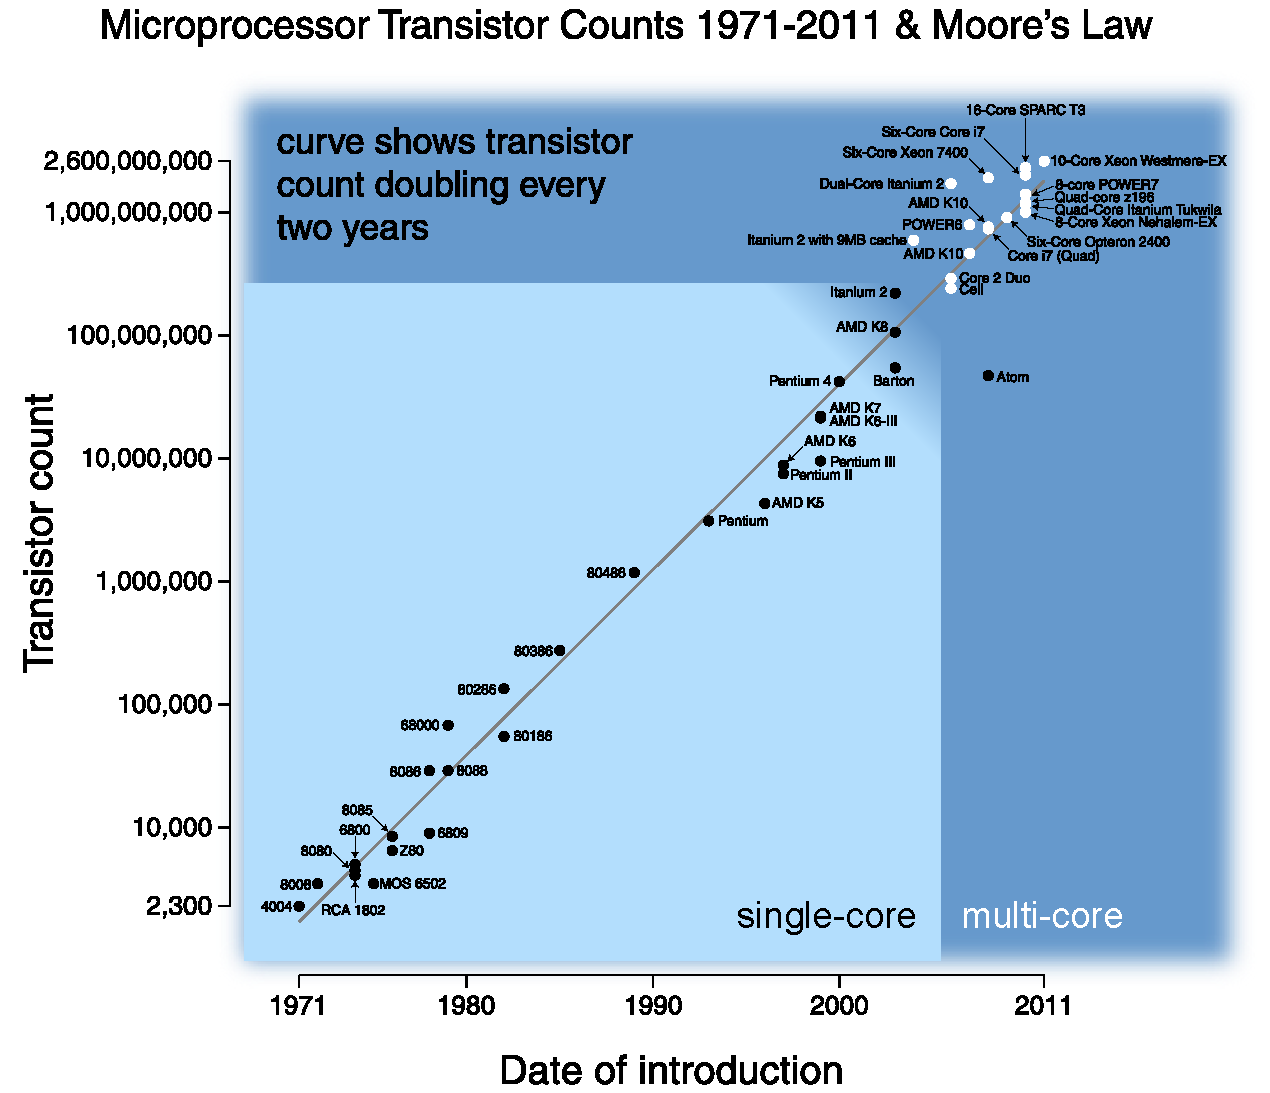
\includegraphics[width=\plotwidth]{images/moore-law.pdf}
   \caption{Cantidad de transistores en procesadores emblem\'aticos desde 1971}
   \label{moore-law}
\end{figure}

Sin embargo, a medida que los transistores disminuyen su tama\~no, aumentan su disipaci\'on t\'ermica por unidad de superficie.
Esto limita la cantidad que se pueden ubicar en un circuito sin producir que este se comporte de manera err\'atica.
El mismo motivo impide el crecimiento de frecuencia de reloj, uno de los principales motores de avance en eficiencia.
Los problemas t\'ermicos han implicado que desde el 2002, la tasa de crecimiento de la performance de los monoprocesadores haya disminuido a un 20\% anual.
Consecuentemente, los principales fabricantes de procesadores han modificado el enfoque de investigaci\'on y dise\~no, empezando a hacerse m\'as y m\'as com\'un el uso de m\'ultiples procesadores por chip.

La preocupaci\'on por la disipaci\'on y el consumo energ\'etico insustentables han sido motivadores de dise\~nos con menor frecuencia de clock, pero aprovechando las a\'un crecientes densidades de transistores para incrementar las unidades de soporte.
Esta estrategia ha resultado en que, en un CPU moderno, menos del 20\% de todos los transistores disponibles se utilicen para realizar c\'alculos.

Adicionalmente, las mejoras de performance debidas al paralelismo a nivel de instrucci\'on (mediante t\'ecnicas como ejecuci\'on fuera de orden, ejecuci\'on especulativa, \textit{pipelining}, etc.) han sido progresivamente menores.
Actualmente, los esfuerzos invertidos en ese \'area se han concentrado en el paralelismo a nivel de datos (vectorizaci\'on) y paralelismo a nivel de tareas (multiprocesadores)~\cite{HennessyPatterson}.

Este enfoque en dise\~no de arquitecturas hacia otros tipos de paralelismo puede verse tanto en nuevos productos en las l\'ineas establecidas (por ejemplo los procesadores Intel i3, i5 e i7) as\'i como tambi\'en en nuevos desarrollos que apunten a c\'omputo de alta performance.
La revalorizaci\'on de las placas gr\'aficas (GPUs) para problemas de c\'omputo intensivo, y los desarrollos nuevos como la arquitectura MIC (\textit{Many Integrated Core Architecture}) de Intel son claros ejemplos de esta tendencia.

El impacto de este enfoque hacia m\'ultiples hilos de ejecuci\'on en paralelo en el desarrollo de aplicaciones es significativo.
En simulaciones para las \'areas de biolog\'ia, medicina, qu\'imica o meteorolog\'ia es de invaluable utilidad minimizar los tiempos de ejecuci\'on, para permitir mejores implementaciones de los modelos utilizados, permitiendo realizar predicciones de mayor calidad.
Aprovechar las nuevas arquitecturas multiprocesador requiere modificaciones en el c\'odigo que resultan no triviales, a diferencia del crecimiento en velocidad de \textit{clock} que no requer\'ia modificaciones en el dise\~no del programa.
Los intentos de escribir programas que conviertan programas seriales (dise\~nados para un solo procesador) a paralelos, en lenguajes de prop\'osito general como C, C++ o Fortran, han sido relativamente infructuosos~\cite{Pacheco}.

Existen sin embargo herramientas que realizan transformaciones de c\'odigo fuente serial a c\'odigo fuente con anotaciones de paralelizaci\'on autom\'aticas (usando librer\'ias de paralelizaci\'on asistida como OpenMP para las anotaciones).
Ejemplos de estas herramientas incluyen Par4All~\cite{Par4AllThesis} y Cetus~\cite{CetusPaper}. Estas herramientas pretenden adem\'as generar c\'odigo para aceleradores especiales como GPGPUs.

El resultado es que es necesario trabajo a nivel de escritura del \textit{software} para utilizar m\'ultiples procesadores.
La aparici\'on de nuevas herramientas ayudan al programador en esta tarea.
Un ejemplo de esto es \nvidia CUDA~(\textit{Compute Unified Device Architecture}), que provee un lenguaje de programaci\'on unificado para el desarrollo de aplicaciones que exploten la arquitectura de unidades GPGPU~(\textit{General Purpose Graphical Processing Units}).
Otros ejemplos los podemos ver en APIs y librer\'ias unificadas de desarrollo como OpenMP o MPI~(\textit{Message Passing Interface}), trabajando conjuntamente con compiladores
optimizantes como Intel ICC y PGI Fortran.

Estas herramientas, si bien resultan en una asistencia muy importante para el programador, no son \textit{silver bullets}.
Todav\'ia la divisi\'on del trabajo es inherente al problema a resolver, en base a las dependencias de las tareas a realizar para la soluci\'on del mismo.
Realizar esta divisi\'on es una labor que, hasta el d\'ia de hoy, se relega en el programador especializado.

En este trabajo, buscaremos comparar distintas arquitecturas de hardware y c\'omo las caracter\'isticas espec\'ificas de la simulaci\'on qu\'imica a realizar permiten o impiden paralelizaci\'on de trabajo empleando los distintos recursos que cada arquitectura provee.
